\newSection{Method}

%---------------------------------------------------------
\subsection{HairStep Representation}
%---------------------------------------------------------

\begin{frame}[t]{HairStep Representation}
    \emph{HairStep} is defined as $\mathbf{H} = \{\mathbf{O}, \mathbf{D}\}$ for each input image $\mathbf{I} \in \mathbb{R}^{W \times H \times 3}$, where:
    \begin{itemize}
        \item $\mathbf{O} \in \mathbb{R}^{W \times H \times 3}$ is the \textbf{Strand Map}.
        \item $\mathbf{D} \in \mathbb{R}^{W \times H \times 1}$ is the \textbf{Depth Map}.
    \end{itemize}

    \vspace{5pt}
    \begin{figure}[t]
        \centering
        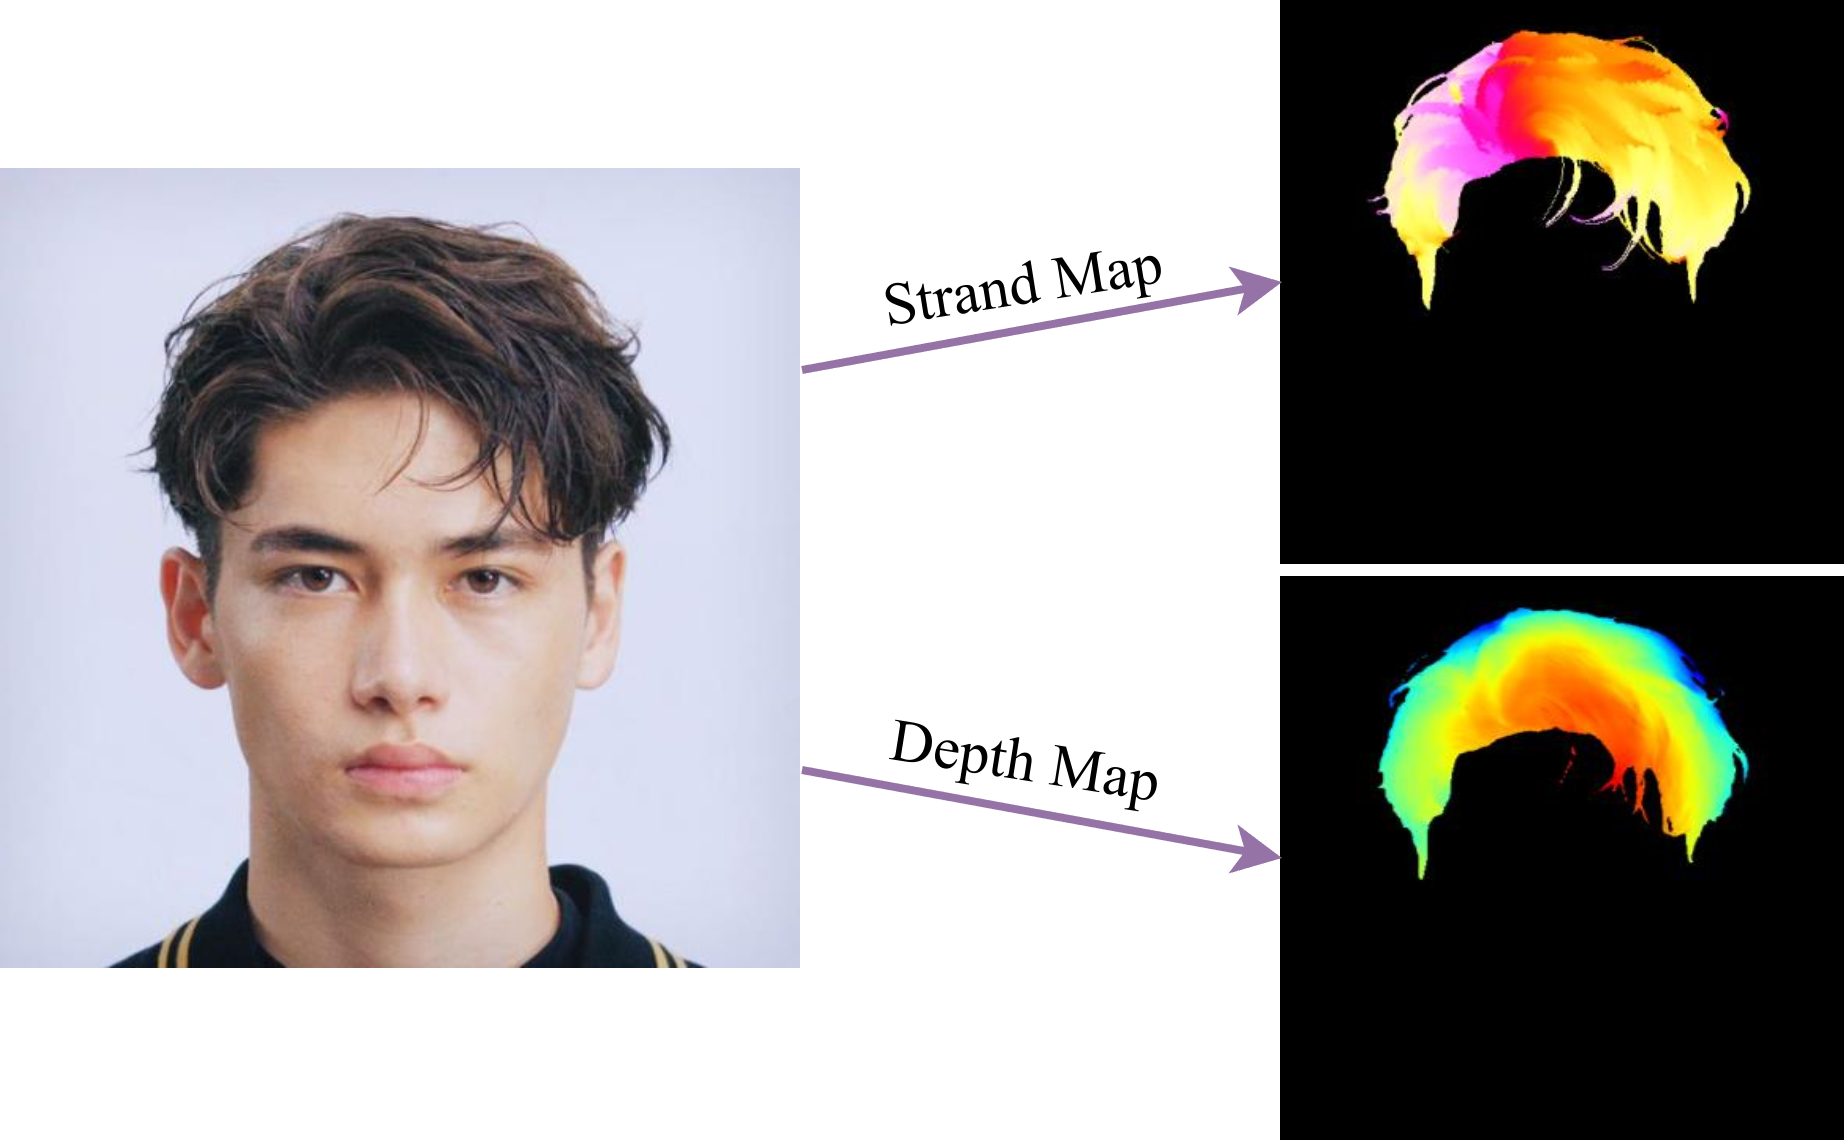
\includegraphics[width=0.45\textwidth]{assets/figures/method/hairstep.png}
        \caption{Example of the \emph{HairStep} representation.}
        \label{fig:hairstep_rep}
    \end{figure}
\end{frame}

%---------------------------------------------------------
\begin{frame}[t]{Strand Map Definition}
    The \textbf{Strand Map} $\mathbf{O} \in \mathbb{R}^{W \times H \times 3}$ is defined at each pixel $x$ as:
    \begin{equation}
        \mathbf{O}(x) = \bigl(\mathbf{M}(x),\; \tfrac{\mathbf{O}_{\mathrm{2D}}(x)}{2} + 0.5\bigr),
        \label{eq:strand_map}
    \end{equation}
    where:
    \begin{itemize}
        \item $\mathbf{M}(x) \in \{0, 1\}$ is the hair mask indicating hair regions ($1$) and background ($0$).
        \item $\mathbf{O}_{\mathrm{2D}}(x) \in \mathbb{R}^2$ is the unit vector of 2D hair-growth orientation at pixel $x$.
    \end{itemize}

    \vspace{5pt}
    \begin{figure}[t]
        \centering
        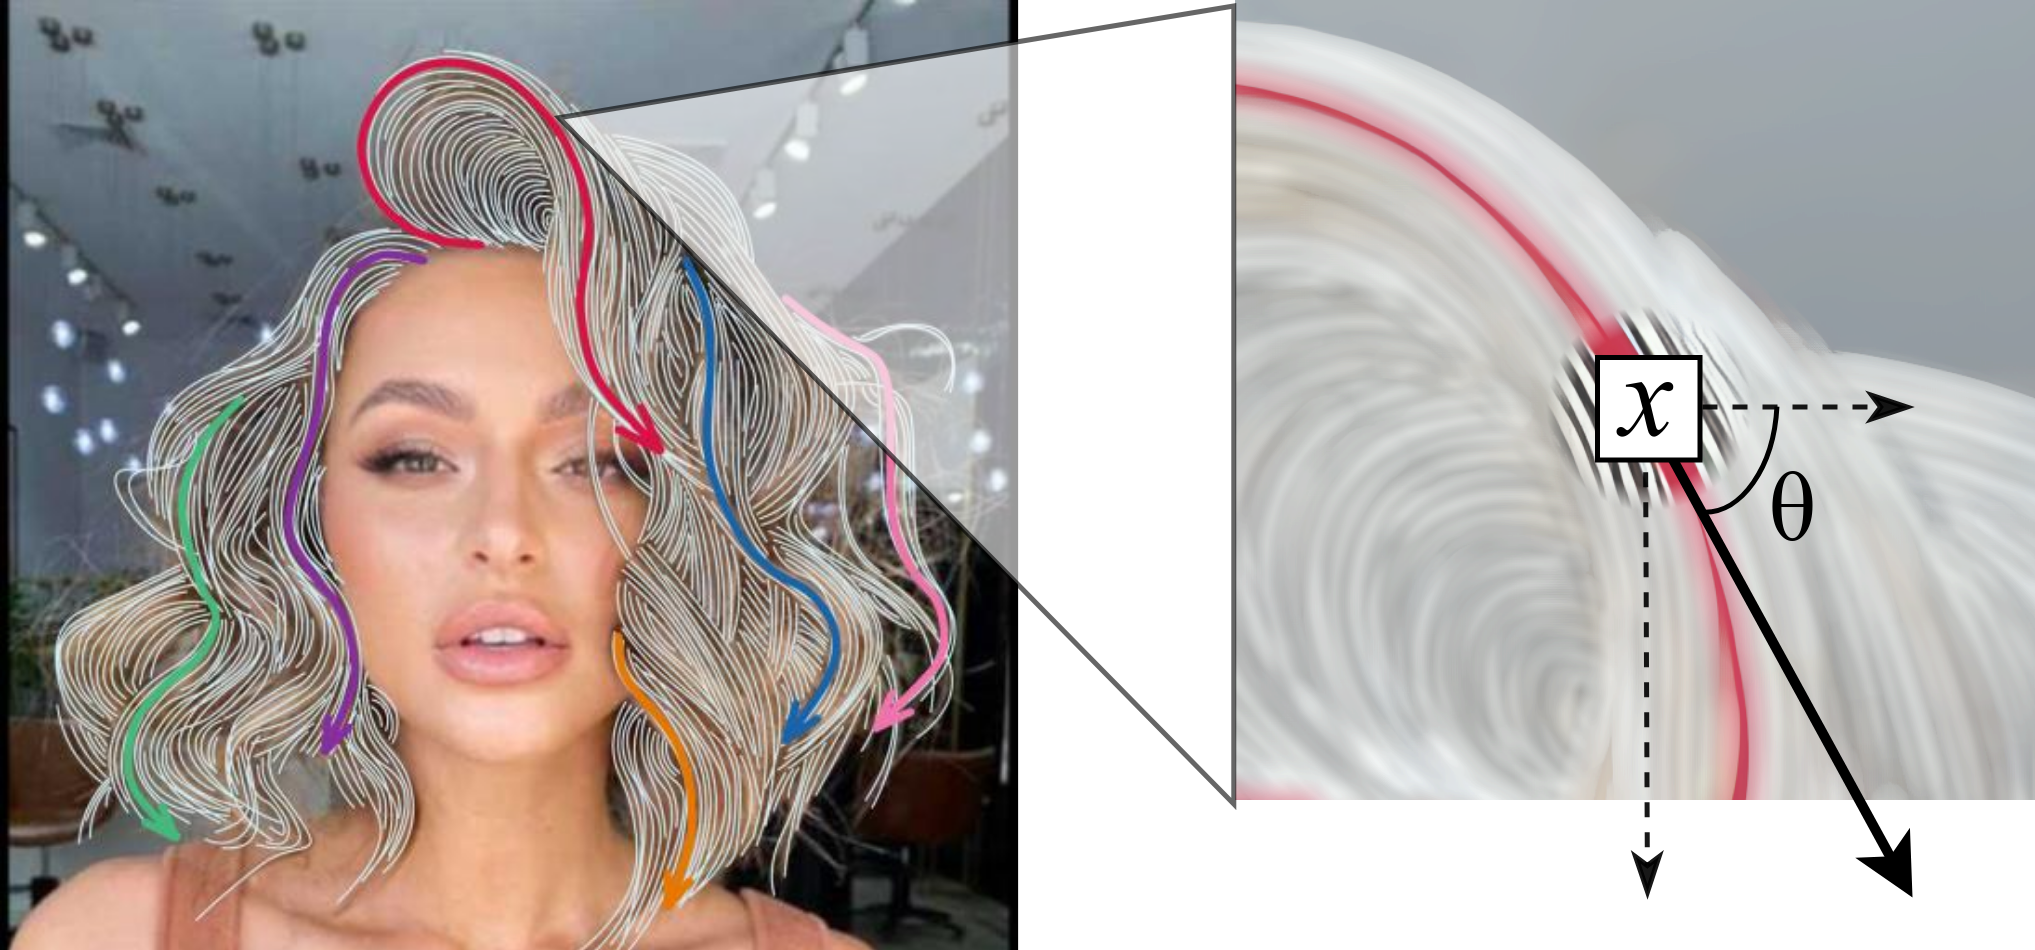
\includegraphics[width=0.45\textwidth]{assets/figures/method/hisa/o_2d.png}
        \caption{Visualization of $\mathbf{O}_{\mathrm{2D}}(x)$, where 
        $\mathbf{O}_{\mathrm{2D}}(x) = \begin{bmatrix}\cos(\theta) \\ -\sin(\theta)\end{bmatrix}$.}
        \label{fig:o_2d_example}
    \end{figure}
\end{frame}

%---------------------------------------------------------
\begin{frame}[t]{Depth Map Definition}
    The \textbf{Depth Map} $\mathbf{D} \in \mathbb{R}^{W \times H \times 1}$ defines relative depth differences among hair strands.

    \vspace{5pt}
    \begin{itemize}
        \item Each pixel $\mathbf{D}(x) \in [0, 1]$:
        \begin{itemize}
            \item $\mathbf{D}(x) = 0$: Farthest from the camera (background or distant strands).
            \item $\mathbf{D}(x) = 1$: Closest to the camera.
        \end{itemize}
    \end{itemize}

    \vspace{5pt}
    \begin{figure}[t]
        \centering
        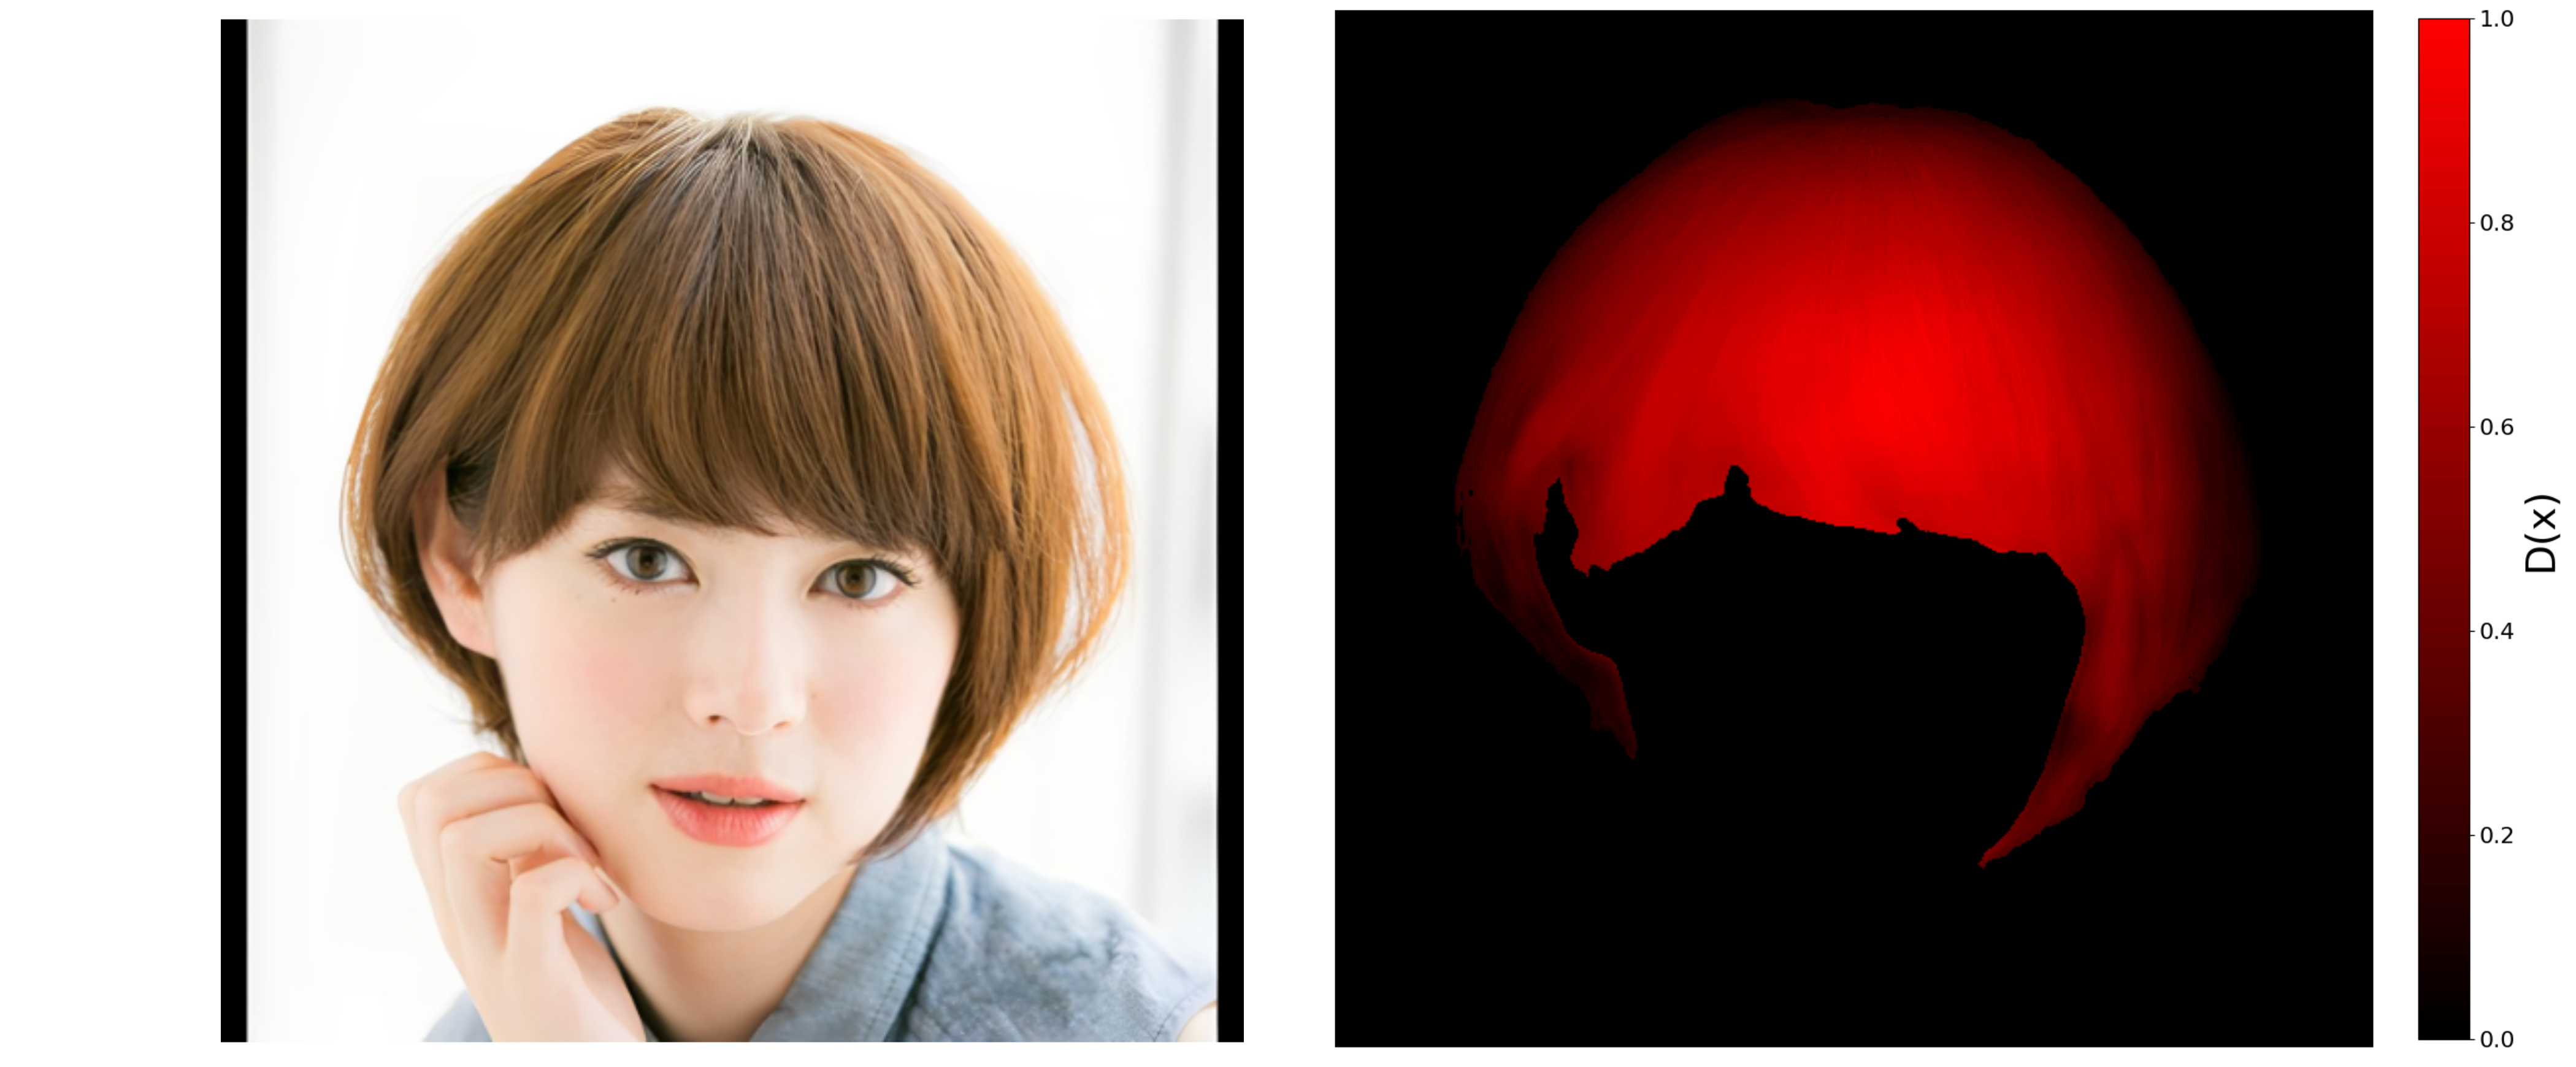
\includegraphics[width=0.55\textwidth]{assets/figures/method/depth-map/depth-map.png}
        \caption{Example of the depth map $\mathbf{D}(x)$.}
        \label{fig:depth_map_example}
    \end{figure}
\end{frame}

%---------------------------------------------------------
\subsection{Pipeline Overview}
%---------------------------------------------------------

\begin{frame}[t]{Method Overview}
    \begin{figure}[t]
        \centering
        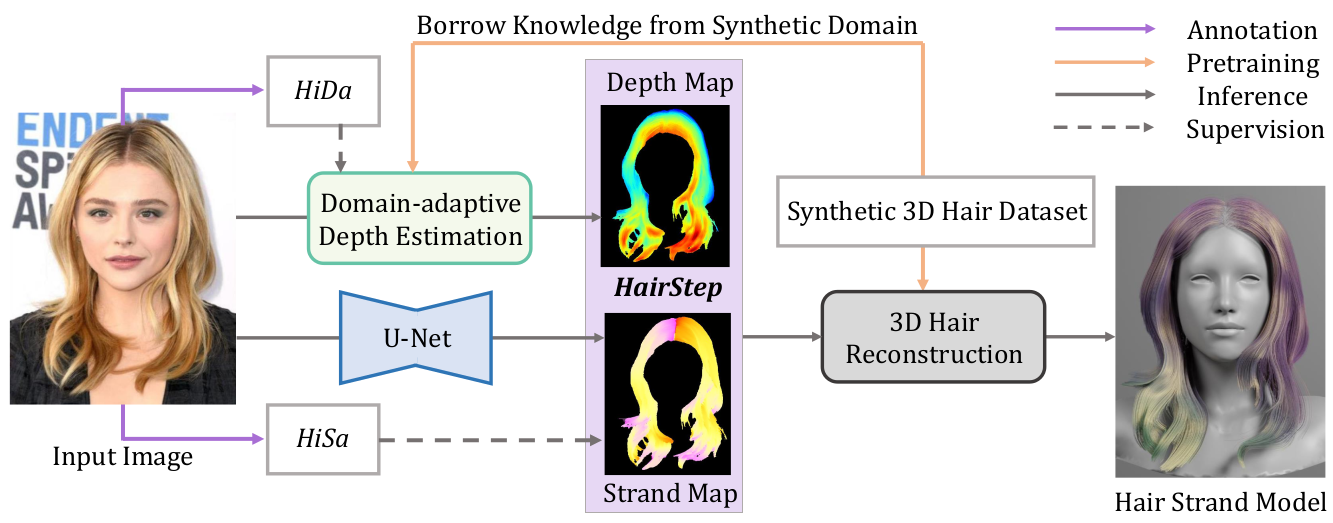
\includegraphics[width=0.95\textwidth]{assets/figures/method/overview.png}
        \caption{Pipeline of single-view 3D hair reconstruction using \emph{HairStep}.}
        \label{fig:overview}
    \end{figure}
\end{frame}

%---------------------------------------------------------
\begin{frame}[t]{Method Overview}
    The pipeline consists of three main components:
    \begin{enumerate}
        \item \textbf{Strand Map Extraction and Prediction}
        \begin{itemize}
            \item Extract strand maps from real images using the \emph{HiSa} dataset.
            \item Train a network to predict strand maps from input images.
        \end{itemize}

        \item \textbf{Domain-Adaptive Depth Estimation}
        \begin{itemize}
            \item Estimate relative depth from real images using the \emph{HiDa} dataset.
            \item Employ domain adaptation techniques to refine depth estimation.
        \end{itemize}

        \item \textbf{3D Hair Reconstruction}
        \begin{itemize}
            \item Reconstruct 3D hair strands from the predicted strand and depth maps.
            \item Utilize implicit fields for volumetric hair representation.
        \end{itemize}
    \end{enumerate}
\end{frame}

%---------------------------------------------------------
\subsection{Strand Map Extraction and Prediction}
%---------------------------------------------------------

\begin{frame}[t]{Strand Map Extraction}
    Extracting strand maps is crucial for learning-based 3D hair modeling.

    \vspace{5pt}

    \textbf{Approaches for Strand Map Extraction:}
    \begin{itemize}
        \item \textbf{Synthetic Data:} Use rendering techniques (e.g., Soft Rasterizer~\cite{liu2019softras}).
        \item \textbf{Real Data:} Use a U-Net architecture trained on the \emph{HiSa} dataset.
    \end{itemize}
\end{frame}

%---------------------------------------------------------
\begin{frame}[t]{HiSa Dataset}
    The \emph{HiSa} dataset provides strand maps for real images.

    \vspace{5pt}

    \textbf{Dataset Details:}
    \begin{itemize}
        \item \textbf{Collection:} 1,250 high-resolution portrait images.
        \item \textbf{Annotation Process:}
        \begin{itemize}
            \item Professional artists draw directional vector curves from hair roots to ends.
            \item Vector strokes are colored according to Eq.~\ref{eq:strand_map}.
            \item Colored strokes are interpolated to form dense strand maps.
        \end{itemize}
        \item \textbf{Statistics:} On average, 300 strokes per portrait are annotated.
    \end{itemize}
\end{frame}

%---------------------------------------------------------
\begin{frame}{HiSa Dataset Visualization}
    \begin{figure}[h]
        \centering
        \includegraphics[width=0.95\textwidth]{assets/figures/method/hisa/hisa.png}
        \caption{Strand map extraction steps:
        (a) Portrait image, (b) Annotated vector strokes, (c) Colored strokes, (d) Final strand map.}
        \label{fig:hisa}
    \end{figure}
\end{frame}

%---------------------------------------------------------
\begin{frame}{Strand Map Prediction Pipeline}
    \begin{figure}[h]
        \centering
        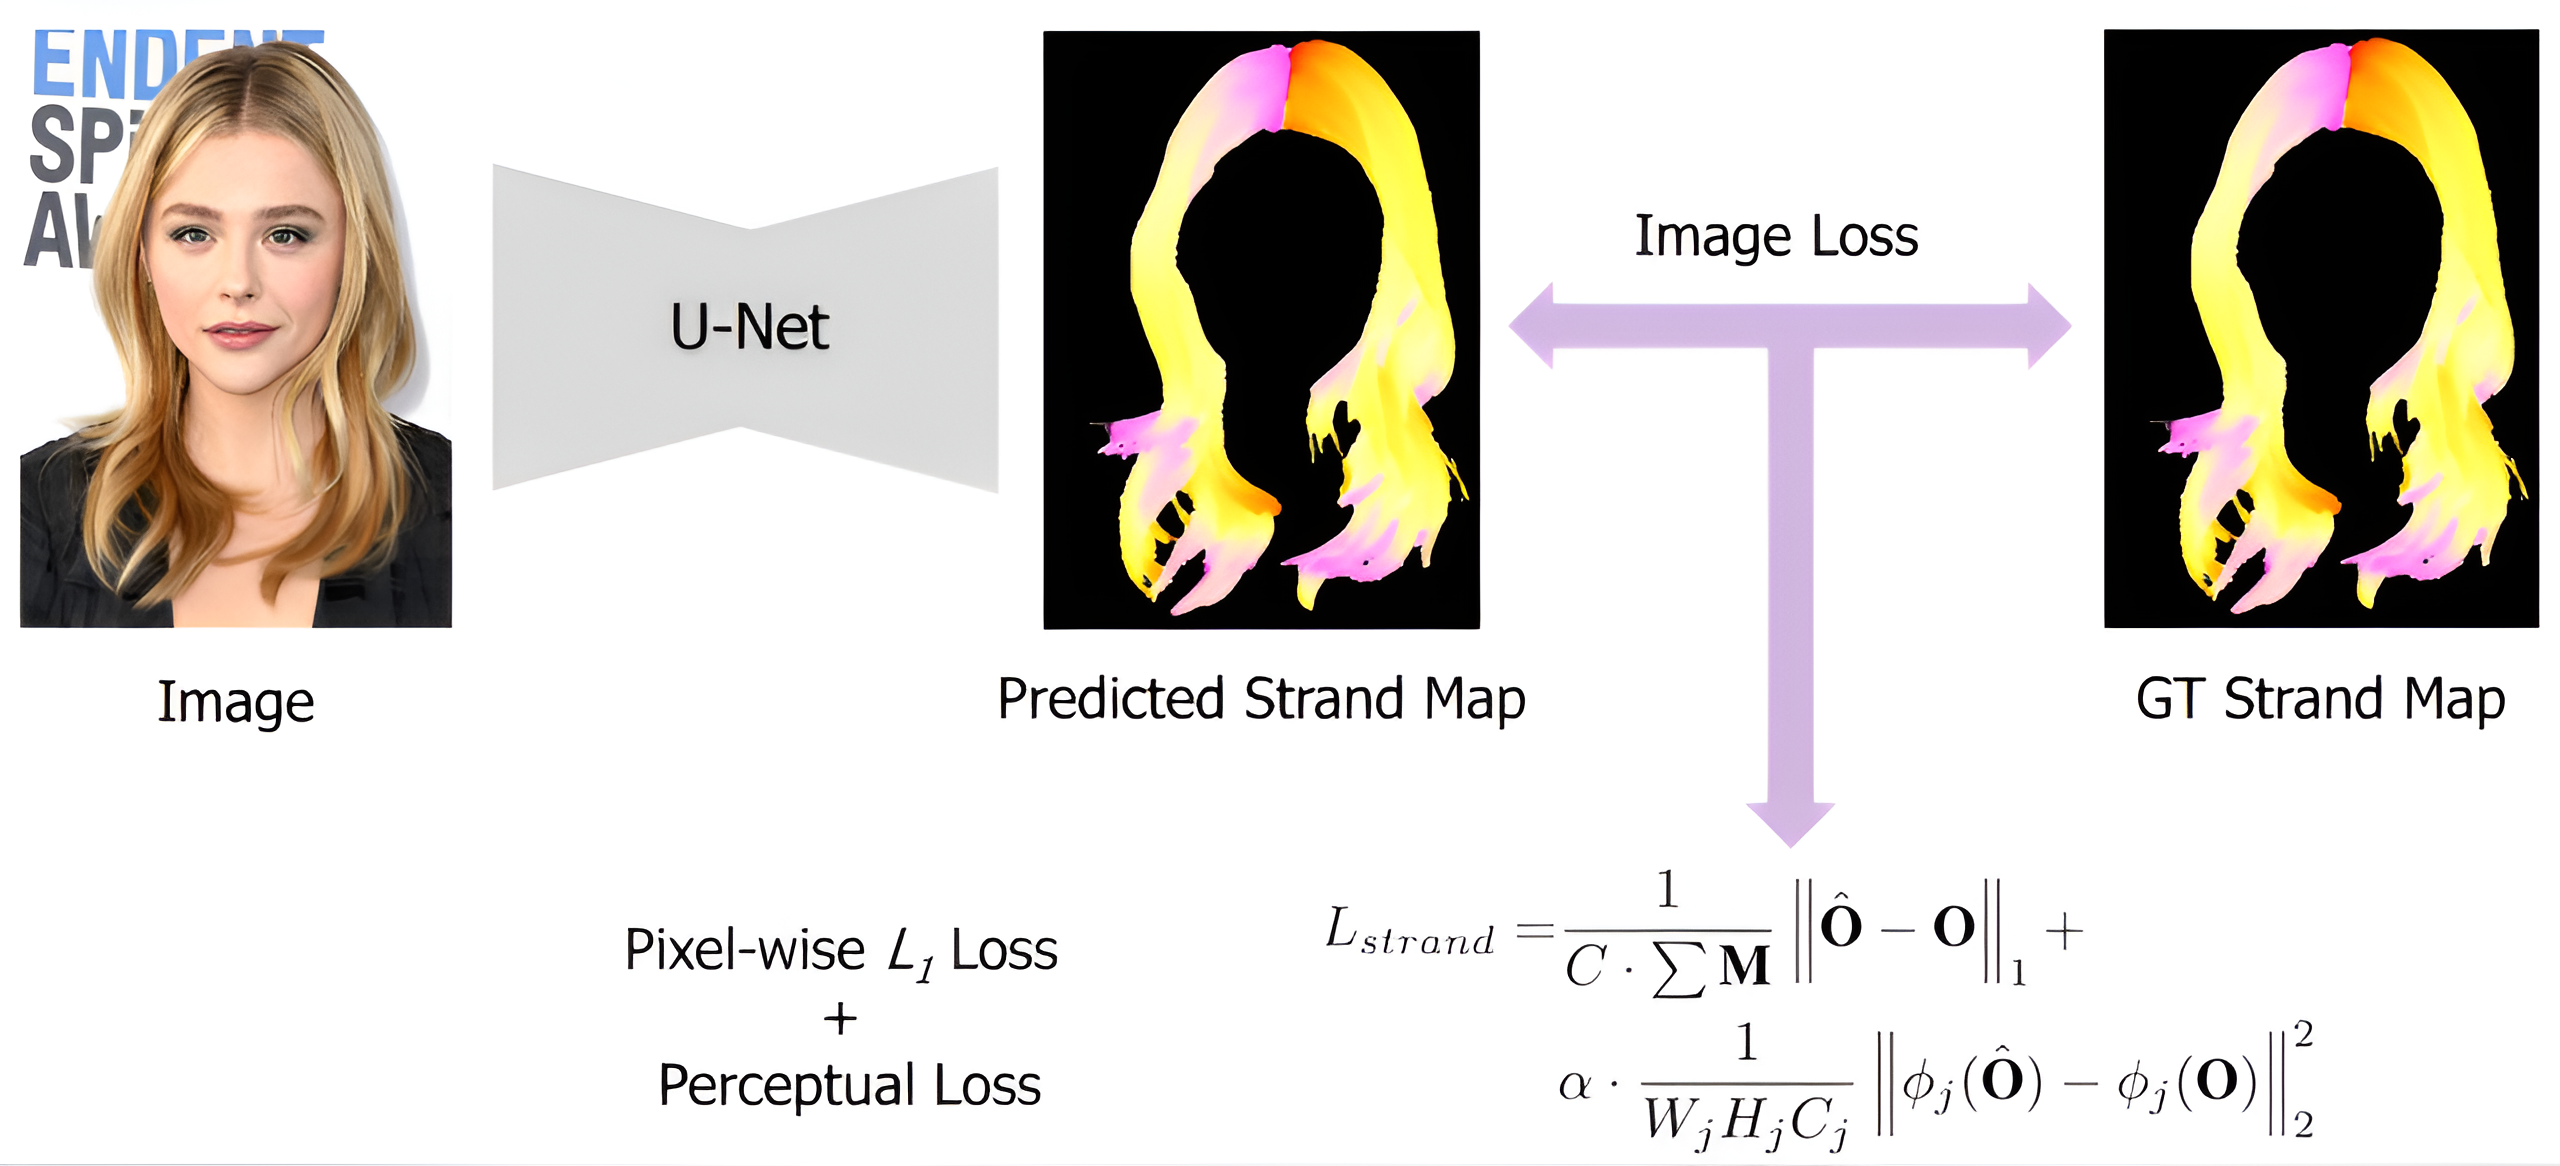
\includegraphics[width=0.95\textwidth]{assets/figures/method/strand/prediction.png}
        \caption{Pipeline for strand map prediction using a U-Net architecture.}
        \label{fig:strand-map-prediction}
    \end{figure}
\end{frame}

%---------------------------------------------------------
\subsection{Depth Estimation and HiDa Dataset}
%---------------------------------------------------------

\begin{frame}[t]{Relative Depth Estimation}
    Inspired by the depth-in-the-wild approach~\cite{chen2016single}, relative depth estimation serves as a weak supervision signal.

    \vspace{5pt}

    \begin{figure}[t]
        \centering
        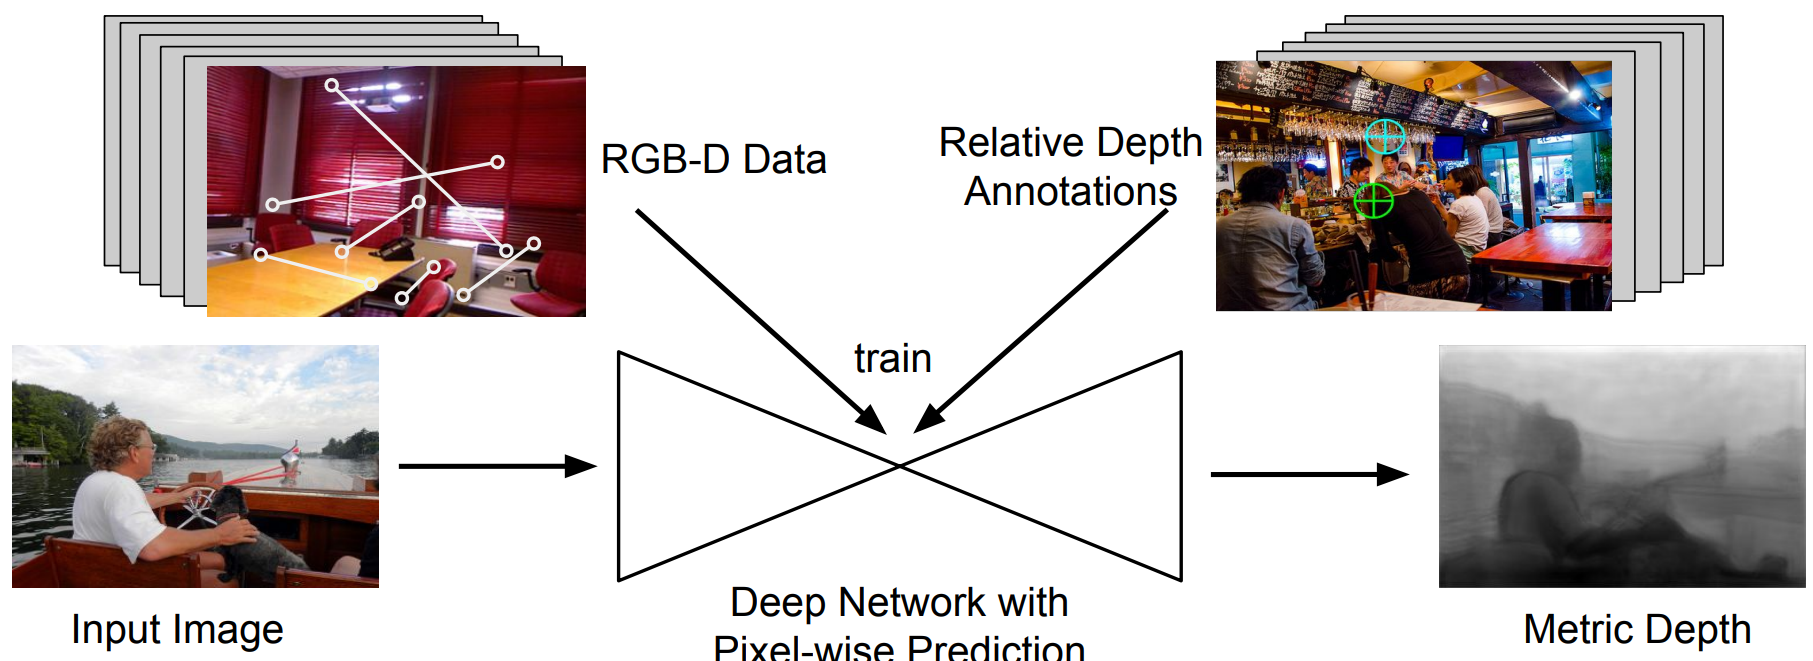
\includegraphics[width=0.85\textwidth]{assets/figures/method/depth/depth-in-the-wild.png}
        \caption{Overview of the depth-in-the-wild pipeline.}
        \label{fig:depth_in_the_wild}
    \end{figure}
\end{frame}

%---------------------------------------------------------
\begin{frame}[t]{HiDa Dataset}
    The \emph{HiDa} dataset provides relative depth annotations for hair regions in real images.

    \vspace{5pt}

    \textbf{Dataset Details:}
    \begin{itemize}
        \item \textbf{Collection:} 1,250 portrait images (same as \emph{HiSa}).
        \item \textbf{Annotation Process:}
        \begin{itemize}
            \item Generate super-pixels within the hair region.
            \item Sample pixel pairs from adjacent super-pixels.
            \item Present each pair to annotators to label which point is closer to the camera.
        \end{itemize}
        \item \textbf{Statistics:}
        \begin{itemize}
            \item On average, 140 pairs per portrait.
            \item Total of 129,079 annotated pixel pairs.
        \end{itemize}
    \end{itemize}
\end{frame}

%---------------------------------------------------------
\begin{frame}{HiDa Dataset Visualization}
    \begin{figure}[h]
        \centering
        \includegraphics[width=0.8\textwidth]{assets/figures/method/hida/superpixel.png}
        \caption{Example of super-pixels generated for the \emph{HiDa} dataset.}
        \label{fig:hida-superpixel}
    \end{figure}
\end{frame}

%---------------------------------------------------------
\begin{frame}{Domain-Adaptive Depth Estimation Pipeline}
    \begin{figure}[h]
        \centering
        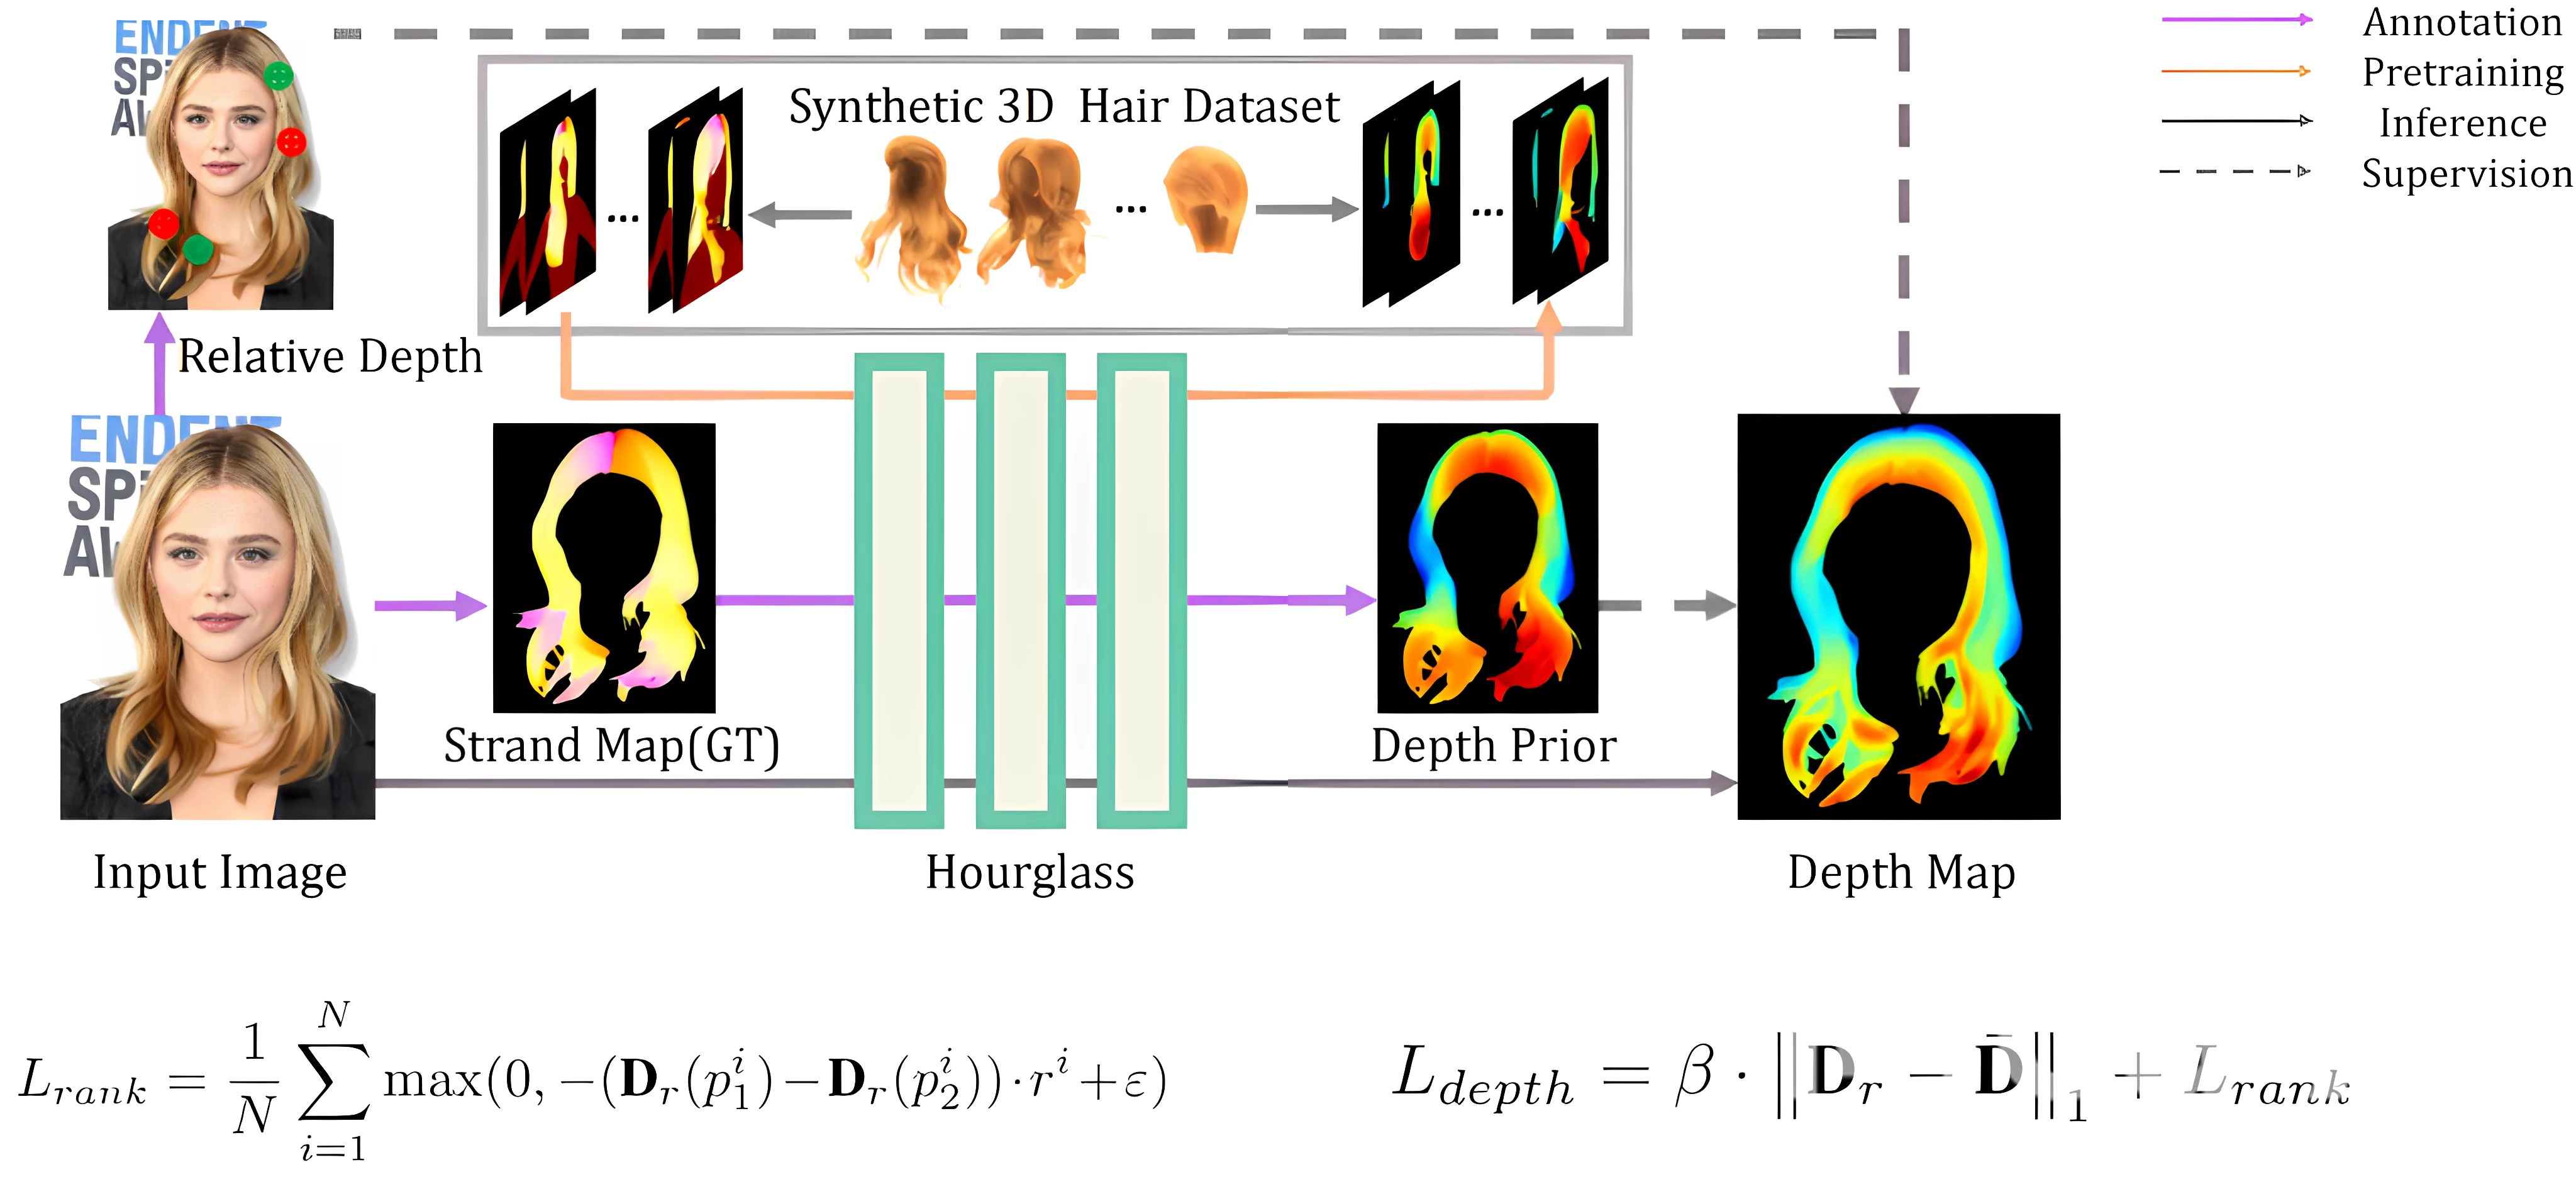
\includegraphics[width=0.9\textwidth]{assets/figures/method/depth/pipeline.png}
        \caption{Overview of the domain-adaptive depth estimation approach.}
        \label{fig:depth_estimation_overview}
    \end{figure}
\end{frame}

%---------------------------------------------------------
\begin{frame}[t]{Depth Estimation Methodology}
    An \textbf{Hourglass Network} is used to predict depth maps from input images.
    \vspace{5pt}
    \begin{itemize}
        \item \textbf{Relative Depth Supervision:} Use margin-based ranking loss with \emph{HiDa} depth pairs.
        \item \textbf{Domain Adaptation:} Enhance depth prediction using synthetic data.
        \item \textbf{Loss Function:} Combine $L_1$ loss and ranking loss:
        \begin{equation}
            L_{\text{depth}} = \beta \|\mathbf{D}_r - \bar{\mathbf{D}}\|_1 + L_{\text{rank}}.
        \end{equation}  
    \end{itemize}

\end{frame}

\begin{frame}{Depth Estimation Methodology}
    \begin{figure}[h]
        \centering
        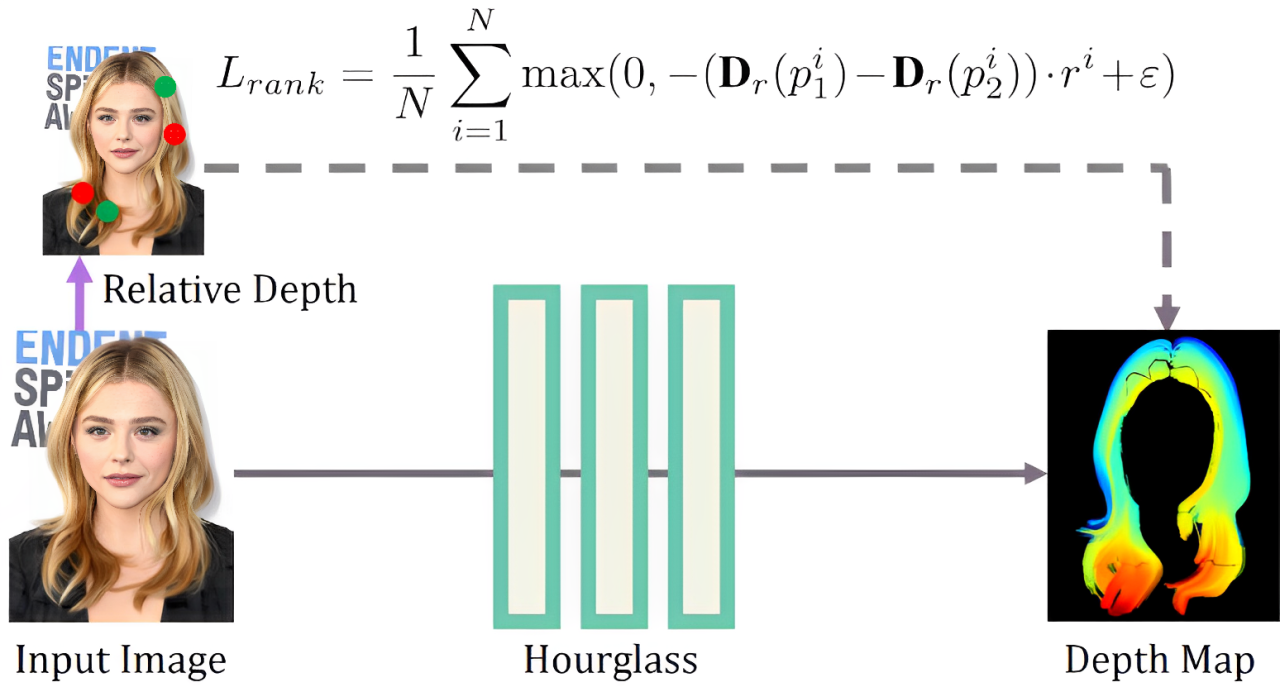
\includegraphics[width=0.8\textwidth]{assets/figures/method/depth/hourglass.png}
        \caption{Hourglass network architecture for depth estimation.}
        \label{fig:hourglass_depth}
    \end{figure}
\end{frame}

%---------------------------------------------------------
\begin{frame}[t]{Challenges in Depth Estimation}
    Training with only ordinal labels can introduce ambiguity and artifacts in depth prediction, resulting in noisy or coarse 3D hair models.

    \vspace{5pt}

    \begin{figure}[t]
        \centering
        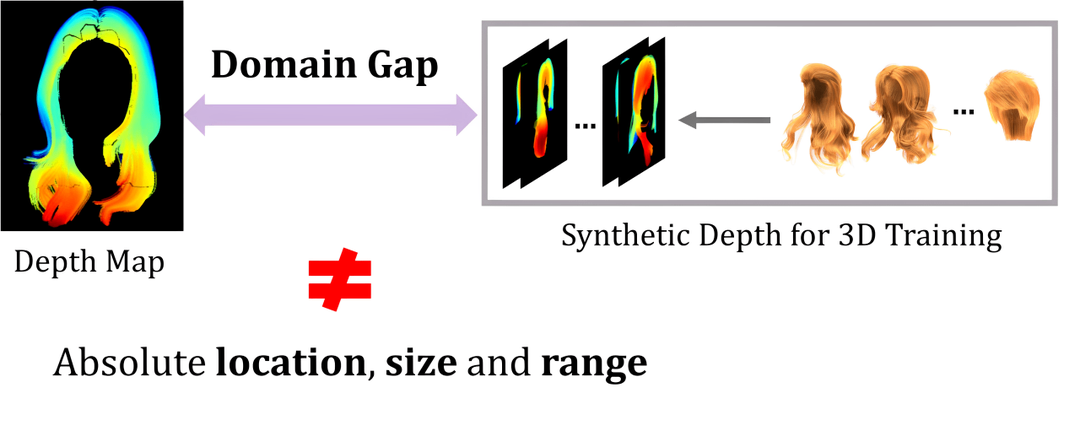
\includegraphics[width=0.6\textwidth]{assets/figures/method/depth/domain-gap.png}
        \caption{Domain gaps and artifacts in predicted depth from ordinal labels.}
        \label{fig:domain_gap}
    \end{figure}
\end{frame}

%---------------------------------------------------------
\begin{frame}[t]{Domain-Adaptive Depth Estimation}
    To mitigate artifacts, domain-adaptive depth estimation pipeline is proposed.

    \vspace{5pt}

    \textbf{Step 1: Pre-training on Synthetic Data}
    \begin{itemize}
        \item \textbf{Network:} Hourglass network (\texttt{Depth\_syn}).
        \item \textbf{Input:} Ground-truth strand maps from synthetic data.
        \item \textbf{Output:} Depth map $\bar{\mathbf{D}}$.
        \item \textbf{Loss:} $L_1$ loss on $\bar{\mathbf{D}}$.
    \end{itemize}

    \vspace{5pt}

    \textbf{Step 2: Training on Real Data}
    \begin{itemize}
        \item \textbf{Network:} Hourglass network (\texttt{Depth\_r}).
        \item \textbf{Input:} Real images with predicted strand maps.
        \item \textbf{Output:} Depth map $\mathbf{D}_r$.
        \item \textbf{Supervision:} Depth prior $\bar{\mathbf{D}}$ from \texttt{Depth\_syn}.
        \item \textbf{Loss:} Combined $L_{\text{depth}}$ as in the loss function.
    \end{itemize}
\end{frame}

%---------------------------------------------------------
\subsection{Single-View 3D Hair Modeling}
%---------------------------------------------------------

\begin{frame}{Single-View 3D Hair Modeling Pipeline}
    \begin{figure}[h]
        \centering
        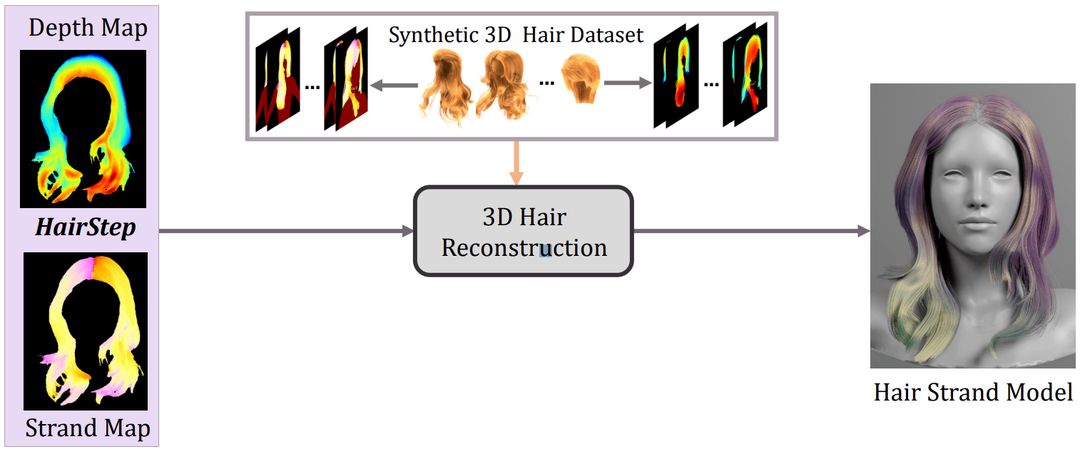
\includegraphics[width=0.9\textwidth]{assets/figures/method/reconstruction.png}
        \caption{Pipeline for single-view 3D hair modeling using \emph{HairStep}.}
        \label{fig:single_view_3d_hair_modeling}
    \end{figure}
\end{frame}

%---------------------------------------------------------
\begin{frame}[t]{Modeling Details}
    \textbf{Objective:} Reconstruct strand-level 3D hair from a single-view portrait image using the \emph{HairStep} representation $\{\mathbf{O}, \mathbf{D}\}$.

    \vspace{5pt}

    \textbf{Key Components:}
    \begin{enumerate}
        \item \textbf{Implicit Representation}
        \begin{itemize}
            \item Predict occupancy and orientation fields in a canonical head space.
            \item Utilize a neural network to model volumetric hair structure.
        \end{itemize}
        \item \textbf{Strand Generation}
        \begin{itemize}
            \item Convert implicit fields into explicit 3D hair strands.
            \item Follow orientation field vectors to grow strands from scalp.
        \end{itemize}
    \end{enumerate}
\end{frame}

%---------------------------------------------------------
\begin{frame}[t]{Implicit 3D Hair Representation}
    \textbf{Why Use Implicit Fields?}
    \begin{itemize}
        \item Efficiently represent complex volumetric structures.
        \item Capture continuous geometry without discretizing every strand.
    \end{itemize}

    \vspace{5pt}

    \textbf{Definitions (Following NeuralHDHair~\cite{wu2022neuralhdhair}):}
    \begin{itemize}
        \item \textbf{Occupancy Field} $f_{\text{occ}}(\mathbf{x}) \in [0,1]$
        \begin{itemize}
            \item Indicates whether point $\mathbf{x}$ is inside the hair volume.
        \end{itemize}
        \item \textbf{Orientation Field} $f_{\text{orient}}(\mathbf{x}) \in \mathbb{R}^3$
        \begin{itemize}
            \item Provides the local hair-growth direction at point $\mathbf{x}$.
        \end{itemize}
    \end{itemize}
\end{frame}

%---------------------------------------------------------
\begin{frame}[t]{Neural Network Prediction (NeuralHDHair*)}
    \textbf{Adapted NeuralHDHair Framework:}

    \vspace{5pt}

    \textbf{Input:}
    \begin{itemize}
        \item Strand map $\mathbf{O}$ (from \emph{HairStep}).
        \item Depth map $\mathbf{D}$ (from domain-adaptive depth estimation).
    \end{itemize}

    \vspace{5pt}

    \textbf{Output:}
    \begin{itemize}
        \item Implicit occupancy field $f_{\text{occ}}(\mathbf{x})$.
        \item Implicit orientation field $f_{\text{orient}}(\mathbf{x})$.
    \end{itemize}

    \vspace{5pt}

    \textbf{Modifications:}
    \begin{itemize}
        \item \emph{No Luminance Map}: Exclude luminance to reduce domain gap from lighting variations.
        \item \emph{Omit GrowingNet}: Focus on direct strand generation from implicit fields.
    \end{itemize}
\end{frame}

%---------------------------------------------------------
\begin{frame}[t]{Hair Strand Generation Process}
    After predicting the implicit fields, hair strands are generated from the scalp.

    \vspace{5pt}

    \begin{enumerate}
        \item \textbf{Initialization}
        \begin{itemize}
            \item Place hair roots uniformly on a standard scalp model.
        \end{itemize}
        \item \textbf{Strand Growing}
        \begin{itemize}
            \item From each root, iteratively follow orientation vectors from $f_{\text{orient}}(\mathbf{x})$.
            \item Continue until $f_{\text{occ}}(\mathbf{x}) = 0$ or reaching maximum strand length.
        \end{itemize}
        \item \textbf{Result}
        \begin{itemize}
            \item Obtain a dense set of 3D hair strands (approximately 10,000 strands) that replicate the input hairstyle.
        \end{itemize}
    \end{enumerate}
\end{frame}
